\documentclass[slovak, bachelorpractice]{diploma}

% Packages (balíky makier)
\usepackage[autostyle=true, czech=quotes]{csquotes} % korektná sadzba úvozoviek, podpora pre balík biblatex
\usepackage[backend=biber, style=iso-numeric, alldates=iso]{biblatex} % bibliografia
\usepackage{dcolumn} % stĺpce tabuľky s číselnými hodnotami
\usepackage{subfig} % makrá pre "podobrázky" a "podtabuľky"
\usepackage[csharp]{diplomalst} % sádzanie zdrojákov

% Novy druh tabuľkového stĺpca, v kterom sú čísla zarovnané podľa desetinnej čiarky
\newcolumntype{d}[1]{D{,}{,}{#1}}

% ------------------------------------------------------

% Titulné strany
\ThesisAuthor{Miroslav Kačeriak}
\ThesisSupervisor{Ing. Pavel Dohnálek, Ph.D.}
\SubmissionYear{2021}

% Poďakovanie
\Acknowledgement{Rád by som na tomto mieste poďakoval mojím dvom kolegom, a zároveň zakladateľom herného štúdia Perun Creative, Bc. Jánovi Polachovi a Bc. Jirkovi Vašicovi za prejavenú dôveru, trpezlivosť a ochotu pomôcť počas absolvovania odbornej praxe. Poďakovanie patrí aj mojej priateľke za podnetné rady a postrehy poskytnuté pri písaní tejto práce.}

% Abstrakty
\CzechAbstract{Cieľom tejto bakalárskej práce je popísať absolvovanie odbornej praxe v českom nezávislom hernom štúdiu Perun Creative. Prvá časť si kladie za cieľ charakterizovať štúdio ako také a uviesť základnú klasifikáciu vyvíjaného produktu, teda počítačovej hry Hobo: Tough Life. Následne by som chcel špecifikovať moje pracovné zaradenie v rámci štruktúry spoločnosti a uviesť najdôležitejšie technológie, s ktorými som mal možnosť pracovať. Hlavnú časť tejto práce tvorí popis realizácie konkrétnych projektov. Tie sa týkali najmä vývoja pomocných nástrojov, optimalizácie a prevodu hry na iné platformy, ale aj implementácie konkrétnych herných mechaník. Záver je potom venovaný celkovému zhodnoteniu absolvovanej odbornej praxe so zameraním na uplatnené a novonadobudnuté znalosti a zručnosti.}

\CzechKeywords{Unity engine; C\#; herný vývoj, automatizácia, optimalizácia, vývojárske nástroje}

\EnglishAbstract{Main purpose of this bachelor thesis is to describe how my individual professional practise in czech indie game studio Perun Creative went. First part aims to characterize the studio as such and give a basic classification of the developed product, i.e. the computer game Hobo: Tough Life. Afterwards, I would like to specify my position within the company structure and mention the most important technologies that I had the opportunity to work with. The main part of this thesis is dealing with the implementation of specific projects. These were mainly focused on the creation of development tools, optimization and porting of the game to other platforms, but also the implementation of some game mechanics. The conclusion is then aimed to the overall evaluation of the completed individual professional practice with focus on applied and newly acquired knowledge and skills.}

\EnglishKeywords{Unity engine; C\#; game development, automatisation, optimization, development tools}

% Skratky
\AddAcronym{QA}{Quality Assurance}
\AddAcronym{PC}{Personal Computer}
\AddAcronym{OS}{Operating System}
\AddAcronym{RPG}{Role Playing Game}
\AddAcronym{EOS}{Epic Online Services}
\AddAcronym{CLR}{Common Language Runtime}
\AddAcronym{JIT}{Just-In-Time}
\AddAcronym{IL}{Intermediate Language}
\AddAcronym{XML}{eXtensible Markup Language}
\AddAcronym{WPF}{Windows Presentation Foundation}
\AddAcronym{LFS}{Large File Storage}
\AddAcronym{CI}{Continuous Integration}
\AddAcronym{CD}{Continuous Delivery}
\AddAcronym{CD}{Continuous Deployment}
\AddAcronym{AI}{Artificial intelligence}
\AddAcronym{REST}{Representational State Transfer}
\AddAcronym{API}{Application Programming Interface}
\AddAcronym{JSON}{JavaScript Object Notation}
\AddAcronym{TCP}{Transmission Control Protocol}
\AddAcronym{IP}{Internet Protocol}
\AddAcronym{DLL}{Dynamic Link Library}
\AddAcronym{SSH}{Secure Shell}
\AddAcronym{HTTPS}{Hypertext Transfer Protocol Secure}
\AddAcronym{URL}{Uniform Resource Locator}
\AddAcronym{MTU}{Maximum transmission unit}
\AddAcronym{MSS}{Maximum Segment Size}

% Literatúra
\addbibresource{literature.bib}

% Samotný dokument
\begin{document}
\MakeTitlePages

% Chapter 1
\chapter{Úvod}
\label{sec:Introduction}
V rámci mojej odbornej praxe som dostal možnosť nahliadnuť za oponu herného vývoja v českom nezávislom štúdiu Perun Creative. Nakoľko sa o hry a herný priemysel dlhodobo zaujímam, táto firma a jej tvorba mi bola vopred známa. Aj po prednáške jej dvoch spoluzakladateľov a zároveň programátorov, ktorá sa uskutočnila v priestoroch Vysokej školy báňskej, som bol stále prekvapený vysokou technologickou úrovňou ich prvého projektu. Firmu som chcel kontaktovať so žiadosťou o prácu nezávisle od odbornej praxe, no keď som sa dozvedel, že už niekoho práve na odbornú prax hľadajú, rozhodol som sa to využiť. Pracovnému pohovoru predchádzalo zaslanie programátorského portfólia zloženého zo školských ale aj vlastných prác. Samotný pohovor potom prebiehal online s oboma programátormi Bc. Jánom Polachom a Bc. Jirkou Vašicou, ktorí sa neskôr stali aj mojimi kolegami.

Do firmy som nastúpil na konci životného cyklu projektu, takže som sa nemohol podieľať na vývoji základných herných mechaník. Naopak to znamenalo nutnosť dôkladne sa s celým projektom zoznámiť a pochopiť, ako jednotlivé časti fungujú. Počas praxe som sa podieľal na širokej škále väčších aj menších projektov z oblastí ako sú automatizácia a zefektívnenie vývojárskych či testerských postupov, nasadenie projektu, sieťová infraštruktúra a došlo aj na nejaké tie herné mechaniky. Pri riešení rôznych problémov mi okrem kolegov boli nápomocné aj rôzne teoretické znalosti nadobudnuté počas vysokoškolského štúdia.

% Section 2
\chapter{Popis firmy a pracovného zaradenia}
\label{sec:Firm and me}
% TODO: Overit info u Jirky
\section{Popis firmy a vyvíjaného produktu}
\label{sec:Firm}
Perun Creative s.r.o \cite{Perun} je české nezávislé herné štúdio, ktoré od roku 2015 vyvíja počítačovú hru Hobo: Tough Life \cite{Hobo}.

Hra samotná by sa dala charakterizovať ako RPG z mestského prostredia, kde sa hráč ocitne v role bezdomovca. Ústrednou hernou mechanikou je snaha prežiť v nehostinnom prostredí ulice. Okrem prežitia na hráča čaká aj pútavý príbeh a možnosť hrať kooperatívne až s troma ďalšími hráčmi. Hobo: Tough Life v súčasnosti vychádza na platformách Microsoft Windows a Linux. V budúcnosti sa počíta aj s vydaním na konzolách novej a starej generácie. 

Štúdio Perun Creative má aktuálne dve pobočky. Prvá sa nachádza v Ostrave a jej osadenstvo tvoria výhradne programátori. Pobočka v Olomouci naopak slúži pre menej technicky zameranú časť firmy a síce pre grafika, herného dizajnéra a komunitného manažéra. Štúdio tvorí menej ako desať vývojárov a teda sa svojou veľkosťou radí k menším. Využíva ale aj služby externých pracovníkov prípadne spoločností špecializovaných na testovanie, zvukovú stránku hry a v neposlednom rade aj na preklad textov do rôznych svetových jazykov.
\vspace{-20pt}
\begin{figure}[!htbp]
	\centering
	
\includegraphics[width=0.5\textwidth]{Pictures/perunLogo.pdf}
	\vspace{-35pt}
	\caption{Logo spoločnosti Perun Creative}
	\label{pic:perunLogo}
\end{figure}
\vspace{-20pt}
\section{Pracovné zaradenie}
\label{sec:Me}
Môj prínos štúdiu Perun Creative spočíval hlavne v automatizácií a zefektívnení jednotlivých interných postupov resp. vývoji pomocných nástrojov pre QA oddelenie či ostatných programátorov. Do tejto kategórie by som zaradil projekty ako automatizované zostavenie hry na serveri, zefektívnenie spôsobu nahlasovania jednotlivých problémov prípadne prepracovanie importovania objektov zo starej verzie projektu do novej. K zefektívneniu práce rozhodne prispel aj návrh a implementácia systému klávesových skratiek v hernom engine Unity (bližšie popísanom v sekcií \ref{sec:Unity}) či  program na vytvorenie tzv. \mbox{\enquote{Patch notes}}. Ten bol primárne určený pre testerov, ale do budúcna sa plánuje jeho využitie aj pri informovaní hráčov o novinkách v rámci hry.

Okrem vyššie uvedených projektov som pracoval na novom systéme líhania postavy k spánku, optimalizácií a uvedeniu hry na OS Linux, prevode online časti hry z platformy Steam na platformu EOS a ďalších menších projektoch.
% End of section 2

% Section 3
\chapter{Použité technológie}
\label{sec:Tech}
V nasledujúcej kapitole by som rád v krátkosti zhrnul najdôležitejšie technológie, s ktorými som sa v rámci odbornej praxe stretol. Niektoré som aktívne využíval počas celého obdobia praxe a ich osvojovanie teda prebiehalo organicky. Iné boli špecifické pre konkrétny projekt a danú technológiu som si musel naštudovať počas realizácie projektu. V niektorých prípadoch bolo nutné sa zoznámiť s viacerými technológiami, aby som bol schopný posúdiť ich výhody a nevýhody pri nasadení na konkrétny projekt a vybrať tú správnu. Informácie som poväčšine čerpal z dokumentácií k daným technológiám aj keď nie vždy bola ich úroveň dostatočná.

\section{Programovací jazyk C\# a architektúra .NET}
\label{sec:CsharpDotNet}
C\# \cite{CSharpLang} je objektovo orientovaný, typovo bezpečný programovací jazyk umožňujúci vytvárať aplikácie v .NET ekosystéme. Syntax jazyka C\# vychádza z programovacích jazykov C a C++. Narozdiel od nich ale ponúka vyššiu úroveň abstrakcie. Tá sa prejavuje napríklad na úrovni správy pamäte, čo z jazyka C\# robí voľbu číslo jedna pre začínajúcich programátorov, ktorí by si chceli skúsiť herný vývoj na vlastnej koži.

Architektúra .NET \cite{CSharpLang} potom ponúka okrem virtuálneho stroja CLR, ktorý vykonáva JIT kompiláciu IL kódu do strojových inštrukcií, aj sadu veľmi užitočných knižníc. Tieto knižnice sú organizované do menných priestorov a poskytujú širokú škálu metód vhodných napríklad na prácu so súbormi či sieťovou infraštruktúrou. Veľmi užitočné sú aj nástroje na syntaktickú analýzu XML prípadne platforma Windows Forms, ktorá sa v rámci mojej odbornej praxe vo firme Perun Creative ukázala byť vhodná hlavne na rýchlu tvorbu vývojárskych nástrojov. Kvôli limitáciám tejto technológie sa ale v budúcnosti plánuje prechod na systém WPF.

\section{Unity Engine}
\label{sec:Unity}
Unity Engine \cite{Unity} je platforma pre tvorbu 2D a 3D interaktívneho obsahu renderovaného v reálnom čase. Najväčšie uplatnenie nachádza pri tvorbe malých až stredne veľkých hier, ale je čoraz častejšie využívaný aj v iných odvetviach ako napríklad automobilový či filmový priemysel. Je dostupný pre operačné systémy Windows, Linux a Mac OS. Distribuuje sa zdarma pre študentov alebo jednotlivcov do určitého finančného obratu a za ročný poplatok pre firmy, ktorého výška závisí od rôznych faktorov. Samotný engine je napísaný v jazyku C++ a umožňuje vývoj obsahu v jazyku C\# (bližšie popísanom v sekcií \ref{sec:CsharpDotNet}) pre širokú škálu platforiem, čo znázorňuje \mbox{obrázok \ref{pic:UnityPlatforms}}.

\begin{figure}[!htbp]
	\centering
	
\includegraphics[width=1\textwidth]{Pictures/platforms.png}
	\caption{Platformy podporované Unity engine-om \cite{UnityMultiplatform}}
	\label{pic:UnityPlatforms}
\end{figure}

\section{Verzovací systém Git}
\label{sec:Git}
Git \cite{ProGit} je open source distribuovaný systém na správu verzií vyvinutý Linusom Thorvaldsom a komunitou okolo OS Linux v roku 2005. Umožňuje vrátiť celý projekt alebo vybrané časti do predchádzajúceho stavu, porovnávať zmeny v súboroch, prípadne efektívnu kolaboráciu viacerých vývojárov na spoločnom projekte. Každý člen tímu má k dispozícií kompletný repozitár vrátane histórie jednotlivých súborov, čo pridáva ďalšiu vrstvu ochrany proti výpadkom a poruchám hardvéru. Po každom spustení príkazu \textit{commit} sa uloží aktuálny stav projektu, ktorý je možné spätne dohľadať v prípade nejakého problému.

S gitom je možné pracovať priamo z príkazového riadku ale pre väčšie projekty ako je aj hra Hobo: Tough Life je takýto prístup značne nepraktický a neefektívny. Existuje ale množstvo programov tretích strán, ktoré umožňujú pracovať s gitom z užívateľského rozhrania. Jedným takým je aj nástroj Sourcetree, s ktorým som v rámci mojej odbornej praxe pracoval.

Nakoľko git samotný nie je dobre prispôsobený na správu verzií veľkých súborov, bolo nutné využívať aj jeho rozšírenie Git LFS. 
\section{GitLab CI/CD}
\label{sec:GitLab}
Gitlab CI/CD \cite{Cicd} je súčasť nástroja Gitlab a slúži na vývoj softvéru prostredníctvom kontinuálnych metód ako:
\begin{itemize}
  \item \textbf{Continuous Integration (CI)} - pre každé pridanie zmien do repozitára je možné automatizovane spustiť sadu skriptov, ktorých účelom je projekt zostaviť či otestovať.
  \item \textbf{Continuous Delivery (CD)} - pridáva ďalšiu vrstvu nad rámec CI, umožňuje zostavený a otestovaný kód nasadiť, vyžaduje to ale manuálnu akciu.
  \item \textbf{Continuous Deployment (CD)} - funguje podobne ako Continuous Delivery ale nasadenie prebieha automaticky.
\end{itemize}
Spoločnou filozofiou týchto metód je teda po každej iteratívnej zmene v projekte kód zostaviť, otestovať a prípadne aj nasadiť. Hlavnou výhodou takého prístupu je redukovanie množstva chýb, ktoré by sa inak dostávali do ďalších iterácií a mohli by spôsobiť problémy, keby neboli odchytené v zárodku. Zároveň si kladú za cieľ znížiť potrebu manuálneho zásahu do jednotlivých automatizovaných procesov na minimum.

V rámci mojej odbornej praxe som sa stretol hlavne s metódou CI. Možnosti automatizovaného testovania hry touto metódou sú veľmi obmedzené, o to viac je ale užitočné automatizované zostavenie na serveri. Zostavenie tohto typu projektu na pracovnej stanici je typicky náročne ako časovo tak aj na výpočtový výkon a do značnej miery teda spomaľuje vývoj ako taký. Bolo teda logickým krokom zamerať sa v rámci optimalizácie interných procesov aj na tento aspekt.

\begin{figure}[!htbp]
	\centering
	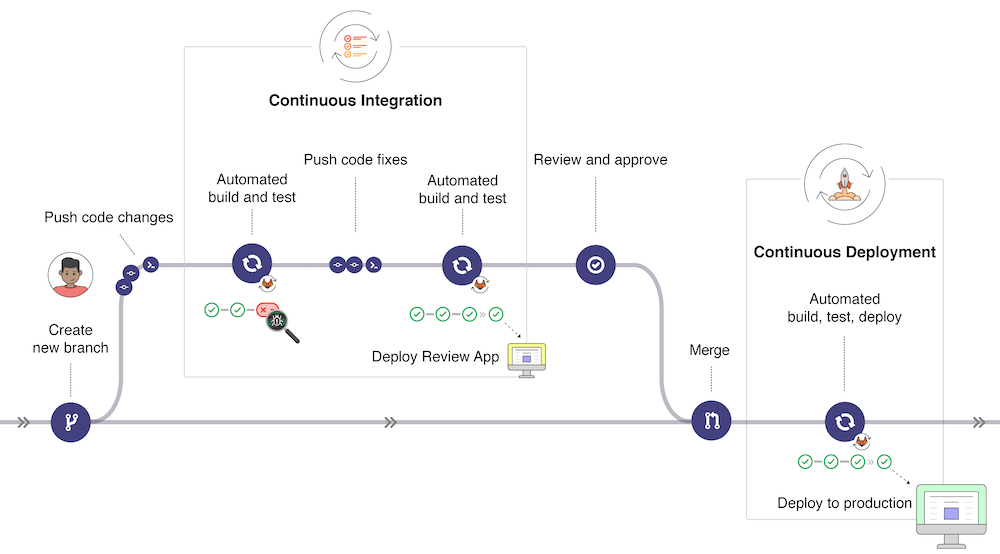
\includegraphics[width=.9\textwidth]{Pictures/gitlab.png}
	\vspace{-15pt}
	\caption{Princíp fungovania Gitab CI/CD \cite{Cicd}}
	\label{pic:Gitlab}
\end{figure}

\section{Epic Online Services}
\label{sec:Eos}
Epic Online Services alebo EOS \cite{Epic} je skupina nástrojov od spoločnosti Epic Games, ktoré sa snažia zjednodušiť a zjednotiť niektoré aspekty herného vývoja naprieč platformami. Typicky sa zameriavajú na kooperatívnu či kompetetívnu zložku hry pre viacerých hráčov, zahŕňajú však aj služby ako nákup herných predmetov za reálne peniaze, zber hráčskych štatistik, prípadne získavanie herných úspechov. Za normálnych okolností je nutné tieto služby implementovať zvlášť takmer pre každú platformu, na ktorú bude hra vychádzať. EOS sú zdarma dostupné pre vývojárov a podporujú širokú škálu platforiem, čo znamená väčšiu slobodu z pohľadu hráča ale aj z pohľadu vývojára. Hráč môže ďalej ťažiť aj z online synchronizácie postupu hrou naprieč viacerými platformami, prípadne z prístupu k úspechom či priateľom z jedného centrálneho miesta. 

Nakoľko sa do budúcna počíta s vydaním hry Hobo: Tough Life na rôzne platformy, ukázalo sa použitie EOS ako veľmi výhodné na náhradu doterajšieho systému pre hru viacerých hráčov. Hlavnou výhodou tohto riešenia by bola vyššie spomínaná multiplatformovosť. V dobe písania tohto textu sa však počíta s nasadením EOS spolu s niektorými službami dostupnými len na konkrétnej platforme.
% End of section 3

% Section 4
\chapter{Zadané projekty a ich riešenia}
\label{sec:Projects}
V tejto kapitole by som rád podrobne prebral konkrétne projekty na ktorých som v rámci mojej odbornej praxe pracoval. Poradie v akom budú prezentované nutne neodzrkadľuje poradie ich vypracovania, ale budú usporiadané do logických celkov podľa typu projektu. 

Čo sa časovej náročnosti týka, nie vždy je možné ju určiť presne nakoľko niektoré z projektov boli vyvíjané inkrementálne podľa spätnej väzby QA oddelenia alebo nových požiadaviek od ostatných programátorov.
%U niektorych prebiehala tvorba inkrementalne a bola zavisla na spatnej vazbe bla bla.

\section{Vývoj pomocných nástrojov pre QA oddelenie a programátorov}
\label{sec:QACode}
\subsection{Evidovanie chybových reportov (Mantis Report)}
\label{sec:Report}
\textbf{Časová náročnosť:} \\ Nasadenie: 8 dní, pridanie ďalšej funkcionality podľa požidaviek: spolu 8 dní.\\
\textbf{Úvod do problému:} \\ Ako som spomenul v sekcií \ref{sec:GitLab} možnosti automatizovaného testovania hry tohto rozsahu sú na rozdiel od bežného softvéru značne obmedzené. Veľké štúdiá si vytvárajú vlastné nástroje založené na AI, nikdy sa to však úplne neobíde bez tvrdej práce ľudí z QA oddelenia ľudovo nazývaných aj ako testeri. Úlohou testera je teda hrať celú hru alebo jej určené časti, nájsť a následne ohlásiť nájdené chyby. 

Takéto ohlásenie chyby je značne neefektívny proces nakoľko na pozadí zahŕňa hneď niekoľko ďalších krokov ako minimalizácia hry, otvorenie stránky so službou Mantis Bug Tracker, nahranie snímky obrazovky a nakoniec aj samotné vyplnenie detailov reportu. Niektoré z týchto detailov sa navyše medzi jednotlivými reportmi nemenia ako napríklad informácie o platforme či operačnom systéme. Ručné vyplnenie reportu znázorňuje obrázok \ref{pic:Mantis}.
Táto neefektívnosť samozrejme priamo úmerne rastie s počtom nájdených chýb, čo môžu byť aj vyššie jednotky denne. Mojou úlohou bolo teda optimalizovať tento postup. \\
\textbf{Navrhované riešenia:} \\ Nakoľko bola toto moja prvá úloha v rámci odbornej praxe, mal som len minimálne skúsenosti s webovými technológiami ako je REST API a celkovo klient-server architektúrou, navrhol som riešenie postavené na nejakom nástroji na automatizovanie webového prehliadača. Takýmto nástrojom je napríklad Selenium WebDriver, s ktorým som sa stretol pri práci na vlastných projektoch. Ten je veľmi obľúbený napríklad pri testovaní webových aplikácií. Dokázal by zapnúť webový prehliadač, či už s užívateľským rozhraním alebo bez, otvoriť požadovanú stránku a vyplniť detaily reportu za užívateľa. V spojení s nejakým vlastným nástrojom na ukladanie snímky obrazovky, prípadne nástrojom, ktorý by testerovi umožnil vypísať zhrnutie či popis reportu priamo v hre by sa naozaj jednalo o relatívne dobré riešenie. Po užívateľovi by to ale vyžadovalo nutnosť inštalácie nejakého konkrétneho prehliadača v požadovanej verzií, aby bola zaistená správna kompatibilita a veľmi pravdepodobne by sa v budúcnosti objavili aj ďalšie problémy s nasadením či používaním. 

Po preskúmaní ďalších možností a následnej porade s kolegami som sa teda rozhodol dať prednosť riešeniu postavenému na už spomínanom REST API a ak by sa to ukázalo ako nerealizovateľné spätne sa vrátiť k môjmu prvému nápadu.
\vspace{-5pt}
\begin{figure}[!htbp]
	\centering
	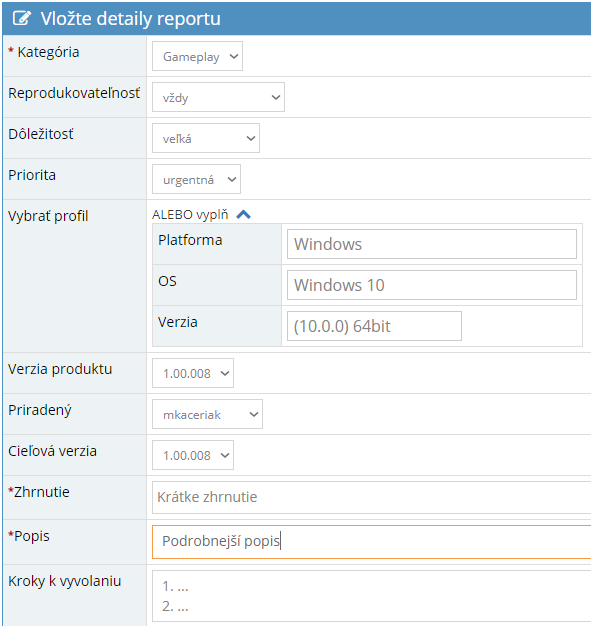
\includegraphics[width=0.7\textwidth]{Pictures/mantis.png}
	\caption{Ručné vloženie reportu do služby Mantis Bug Tracker}
	\label{pic:Mantis}
\end{figure} \\
\textbf{Realizácia:} \\ Pri preskúmavaní možností založených na REST API som narazil na open source projekt MantisSharp \cite{MantisSharp}. Po zoznámení sa s týmto projektom a niekoľkými pokusmi ho \enquote{ohnúť} pre účely môjho projektu som sa rozhodol, že bude jednoduchšie napísať si aplikáciu sám. Využil som k tomu dve triedy z projektu MantisSharp, a síce \textit{RestClient} a \textit{MantisClient}, ktoré som následne ešte ďalej modifikoval. Trieda \textit{RestClient} vykonáva najnižšiu úroveň komunikácie so serverom a síce odosiela GET a POST žiadosti. Trieda \textit{MantisClient} má potom dve úlohy. Na jednej strane prijíma dáta z mojej aplikácie, zabalí ich do formy vhodnej pre transport a následne ich predá triede \textit{RestClient} na odoslanie metódou POST. Na strane druhej transformuje dáta získané zo servera pomocou metódy GET do C\# tried vhodných na následné použitie. Tento postup pridáva určitý level abstrakcie do celej aplikácie.

Problematiku odosielania dát na server som sa rozhodol demonštrovať na pridaní nového reportu vo výpise \ref{src:SendIssue}. Aplikácia vytvorí na základe vstupných dát inštanciu triedy \textit{Issue}, ktorú predá metóde \textit{SendIssue}. Tá ju následne zabalí ako JSON objekt a ďalej predá v metóde \textit{ExecutePost} na finálne odoslanie. Získavanie dát funguje obdobne len opačným smerom. 

Služba Mantis Bug Tracker po úspešnom pridaní nového reportu tento report vráti v odpovedi, čo som ďalej využil na informovanie užívateľa o úspešnom zaevidovaní, ktoré som doplnil o serverom pridelený identifikátor.
\vspace{10pt}
\begin{lstlisting}[label=src:SendIssue,caption={Odoslanie nového reportu na server}]
public int SendIssue(Issue issue) {
	string uri = this.GetUri(issuesUri);
	int id = -1;

	restClient.ExecutePost(uri, () => JsonConvert.SerializeObject(issue),
        reader => {
            string answerFromServer = reader.ReadToEnd();
            JObject obj = JObject.Parse(answerFromServer);
            id = (int)obj["issue"]["id"];
        });

    return id;
}
\end{lstlisting}
Server spočiatku na všetky žiadosti reagoval chybou \enquote{401 Unauthorized}. Po dôkladnom preskúmaní problému sa ukázalo, že chyba je na strane serveru a bolo nutné zasiahnuť do jeho kódu. Nakoľko som k tomuto kódu nemal prístup, požiadal som kolegu, či by mi s tým mohol pomôcť. Ukázalo sa, že server filtroval všetky požiadavky, ktoré sa pokúšali o autorizáciu pomocou tzv. \enquote{Bearer tokenu}. Spoločne sa nám tento problém však podarilo vyriešiť. 

Systém nahlasovania reportov mal byť pôvodne implementovaný ako súčasť hry. To sa ale ukázalo ako problematické z hľadiska zachytávania užívateľského vstupu v Unity engine. V praxi by to znamenalo, že ak by užívateľ popisoval chybu napríklad do nejakého textového poľa, hra samotná by naďalej vykonávala akcie na základe stlačených kláves. Rozhodli sme sa teda začleniť tento systém do už existujúceho vývojárskeho nástroja s názvom HoboThor. Tento nástroj je veľmi komplexný a jeho popis by bol nad rámec tejto kapitoly.

Logika aplikácie bola teda rozdelená do dvoch častí. Časť, s ktorou interaguje užívateľ bola realizovaná ako Windows Forms aplikácia začlenená do nástroja HoboThor a časť, ktorá túto aplikáciu spustí bola implementovaná priamo do hry a vyvolá sa stlačením klávesovej skratky Shift + F11, ak je hra spustená s podporou vývojárskych nástrojov. 

Kontrola, či boli stlačené konkrétne klávesy musí prebiehať každú snímku, aby sa zabezpečilo, že odchytenie prebehne úspešne. Kód zabezpečujúci túto funkcionalitu bol teda vložený do metódy \textit{OnUpdate} triedy \textit{ReportingManager}, čo znázorňuje výpis \ref{src:OnUpdate}. 

Projekt Hobo: Tough Life do veľkej miery stojí na hierarchickej štruktúre tried, tzv. \enquote{Manageroch}, ktorí, ako názov napovedá obstarávajú určité časti aplikácie. Metóda \textit{OnUpdate} triedy \textit{ReportingManager} je teda každú snímku volaná inou triedou, ktorá je vyššie v hierarchickej štruktúre projektu. Na najvyššom stupni hierarchie potom stojí trieda \textit{MainManager}. Tá obsahuje metódu \textit{Update}, ktorá je priamo volaná natívnym C++ kódom enginu Unity a táto metóda potom obsahuje volania metód \textit{OnUpdate} jednotlivých \enquote{Managerov}, ktorí jej náležia.
\vspace{10pt}
\begin{lstlisting}[label=src:OnUpdate,caption={Odchytenie stlačenia klávesovej skratky v spustenej hre}]
public void OnUpdate() {
    if (Keyboard.current.f11Key.wasPressedThisFrame) {
        if (Keyboard.current.leftShiftKey.isPressed) {
            screenSaved = false;
            StartCoroutine(StartCreateReport());
            return;
        }
    }

    if (screenSaved) {
        ZipAndSendToLinkManager();
        screenSaved = false;
    }
}
\end{lstlisting}

Kód vo výpise \ref{src:OnUpdate} teda každú snímku testuje, či bola stlačená klávesa F11 a to práve v tom danom snímku. Toto zabezpečí, že sa blok kódu tejto podmienky vykoná len raz, bez ohľadu na to, ako dlho užívateľ danú klávesu držal stlačenú. Ak je popri tom stlačená aj klávesa Shift, spustí sa tzv. \enquote{Coroutine}. V tomto prípade je ňou mnou definovaná metóda \textit{StartCreateReport}. Výhoda korutiny spočíva v možnosti pozastaviť vykonávanie svojho kódu. Pozastavenie môže byť na programátorom definovanú dobu alebo do doby než nastane určitá udalosť. V tomto prípade bolo tou udalosťou kompletné vykreslenie aktuálneho snímku a to z dôvodu zachytenia tohto snímku ako obrázku.

Metóda \textit{StartCreateReport} má za úlohu zozbierať rôzne dáta o aplikácií alebo systéme, na ktorom je spustená. Ide o dáta ako verzia aplikácie, pozícia a rotácia kamery v momente vyvolania akcie či posledný záznam v logovacom systéme. Tieto dáta sú následne spolu so spomínanou snímkou obrazovky a naposledy uloženým postupom hrou uložené na disk. Zložka, do ktorej sú súbory uložené závisí od toho, či je hra spustená z editoru Unity alebo samostatne. Takéto vetvenie kódu sa realizuje pomocou direktívy UNITY\_EDITOR, ktorá je spolu s ďalšími platformovo závislými direktívami definovaná samotným editorom. Jednoduchý príklad použitia takýchto direktív demonštruje výpis \ref{src:Pragma}. Nakoľko táto zložka obsahuje celú históriu reportov, jednotlivé reporty majú poradové čísla a každý ďalší dostane pridelené poradové číslo o jedna väčšie ako ten predchádzajúci.
\vspace{10pt}
\begin{lstlisting}[label=src:Pragma,caption={Ukážka použitia direktívy UNITY\_EDITOR}]
#if UNITY_EDITOR
	Debug.Log("Editor");                
#else
    Debug.Log("Standalone");             
#endif
\end{lstlisting}

Následne sa logika aplikácie delí na dve vetvy. Prvá obstaráva vytvorenie lokálneho reportu, druhá vzdialeného. Možnosť vzdialeného nahlasovania chýb, teda odoslanie reportu z PC na ktorom hra nie je spustená bola pridaná až neskôr v súvislosti s prevodom hry na iné platformy. Oba spôsoby odoslania reportu potom demonštruje výpis \ref{src:Report}.

Odoslanie reportu na server z lokálneho PC pokračuje vytvorením tzv. \enquote{Mantis argumentu}. Ide o textový súbor, ktorého obsah je cesta k naposledy vytvorenému reportu. Ten je uložený do zložky, kde sa nachádza spúšťací súbor nástroja HoboThor. Následne je tento nástroj spustený a pokiaľ je pri tomto procese prítomný už spomínaný \enquote{Mantis argument}, nespustí sa hlavné okno aplikácie, ale len okno určené na odoslanie reportu. Po prečítaní obsahu je súbor samozrejme zmazaný, aby neovplyvnil ďalšie spustenie nástroja HoboThor.

Pokiaľ ide o odoslanie reportu zo vzdialeného PC ukázala sa ako problematická doba ukladania snímky obrazovky na disk. Kvôli tomuto problému musí aplikácia najskôr počkať na uloženie súboru a až následne vykonávať ďalšie inštrukcie. Toho som docielil jednoduchou slučkou, ktorá sa sama ukončí v prípade nájdenia požadovaného súboru alebo po pretečení určitého času. To slúži ako ochrana pred zacyklením. 

\vspace{10pt}
\begin{lstlisting}[label=src:Report,caption={Vytváranie lokálneho a vzdialeného reportu}]
// Local report
if (HBTLink_Manager.sender_ServerIP == HBTLink_Manager.Instance.LocalIPAddress().ToString()) {
    string exeFile = GameConfiguration.pathConfig.exeFile;
    if (File.Exists(exeFile)) {
        var argFile = GameConfiguration.pathConfig.mantisArguments;

        if (File.Exists(argFile))
            File.Delete(argFile);

        File.WriteAllText(argFile, directoryReport.FullName);
        Application.OpenURL(exeFile);
    }
}
// Remote report
else {
    float time = 0;
    while (time <= maxWaitTime) {
        yield return new WaitForSeconds(.1f);
        time++;
        if (File.Exists(screenFileName)) {
            screenSaved = true;
            yield break;
        }
    }
}
\end{lstlisting}

Na zmenu hodnoty premennej \textit{screenSaved} zareaguje metóda \textit{OnUpdate} z výpisu \ref{src:OnUpdate} a spustí metódu \textit{ZipAndSendToLinkManager}. Tá pomocou knižnice DotNetZip \cite{DotNetZip} prevedie celú zložku s reportom na zip súbor so zachovaním hierarchickej štruktúry podzložiek a súborov. Následne ho prevedie na reťazec s kódovaním base64 a predá triede HBTLink\_Manager na odoslanie do vzdialeného PC. Táto metóda je znázornená vo výpise \ref{src:Zip}. 

Rreťazec je následne pomocou TCP protokolu odoslaný na IP adresu určenú v konfiguračnom súbore alebo vybratú z prednastavených možností vo vývojárskej konzole počas hrania. Na vzdialenom PC musí byť spustený nástroj HoboThor a \enquote{počúvať} na určenom porte. Dáta sú po prijatí uložené do dočasnej zložky poskytovanej operačným systémom pomocou metódy \textit{Path.GetTempPath} v mennom priestore \textit{System.IO} a následne rozbalené. Cesta k tejto zložke je opäť zapísaná do \enquote{Mantis argumentu} a HoboThor je následne automaticky spustený znova. To vyústi k otvoreniu okna určeného na nahlasovanie chýb a načítaniu dát zo zložky s reportom.
\vspace{10pt}
\begin{lstlisting}[label=src:Zip,caption={Metóda ZipAndSendToLinkManager triedy ReportingManager}]
private void ZipAndSendToLinkManager() {
    string pathToZip = directoryReport.FullName + @"\report.zip";

    using (ZipFile zip = new ZipFile()) {
        var files = Directory.EnumerateFiles(directoryReport.FullName, "*.*", SearchOption.AllDirectories);
        foreach (string file in files) {
            if (file.Contains("Characters"))
                zip.AddFile(file, @"\Saves\Characters");
            else if (file.Contains("Worlds"))
                zip.AddFile(file, @"\Saves\Worlds");
            else
                zip.AddFile(file, "");
        }

        zip.Save(pathToZip);
        Debug.Log("Zipped to " + pathToZip);
    }

    if (File.Exists(pathToZip)) {
        string base64zip = System.Convert.ToBase64String(File.ReadAllBytes(pathToZip));
        HBTLink_Manager.Send_MantisReport(base64zip);
        File.Delete(pathToZip);
    }
}
\end{lstlisting}
\vspace{5pt}

Problém tohto postupu bol spočiatku vo veľkosti vyrovnávacej pamäte na strane prijímateľa, teda nástroja HoboThor, ktorá bola poddimenzovaná. Následné testovanie ukázalo, že spoľahlivá veľkosť tejto pamäte začína až na hodnote 2\textsuperscript{20} bytov v závislosti primárne od veľkosti odosielanej snímky obrazovky. Vytvorenie takejto veľkej vyrovnávacej pamäte a následné uloženie všetkých prijatých dát naraz ale nefungovalo na OS Linux. Testovacia aplikácia na tomto systéme zvládla prijať maximálne 14600 bytov. Táto hodnota odpovedá desaťnásobku MTU balíčku preneseného technológiou Ethernet v2 po odčítaní veľkostí TCP a IP hlavičiek. Veľkosť 1460 bytov sa zvykne nazývať aj MSS. Túto problematiku znázorňuje obrázok \ref{pic:Packet}.
\vspace{-50pt}
\begin{figure}[!htbp]
	\centering
	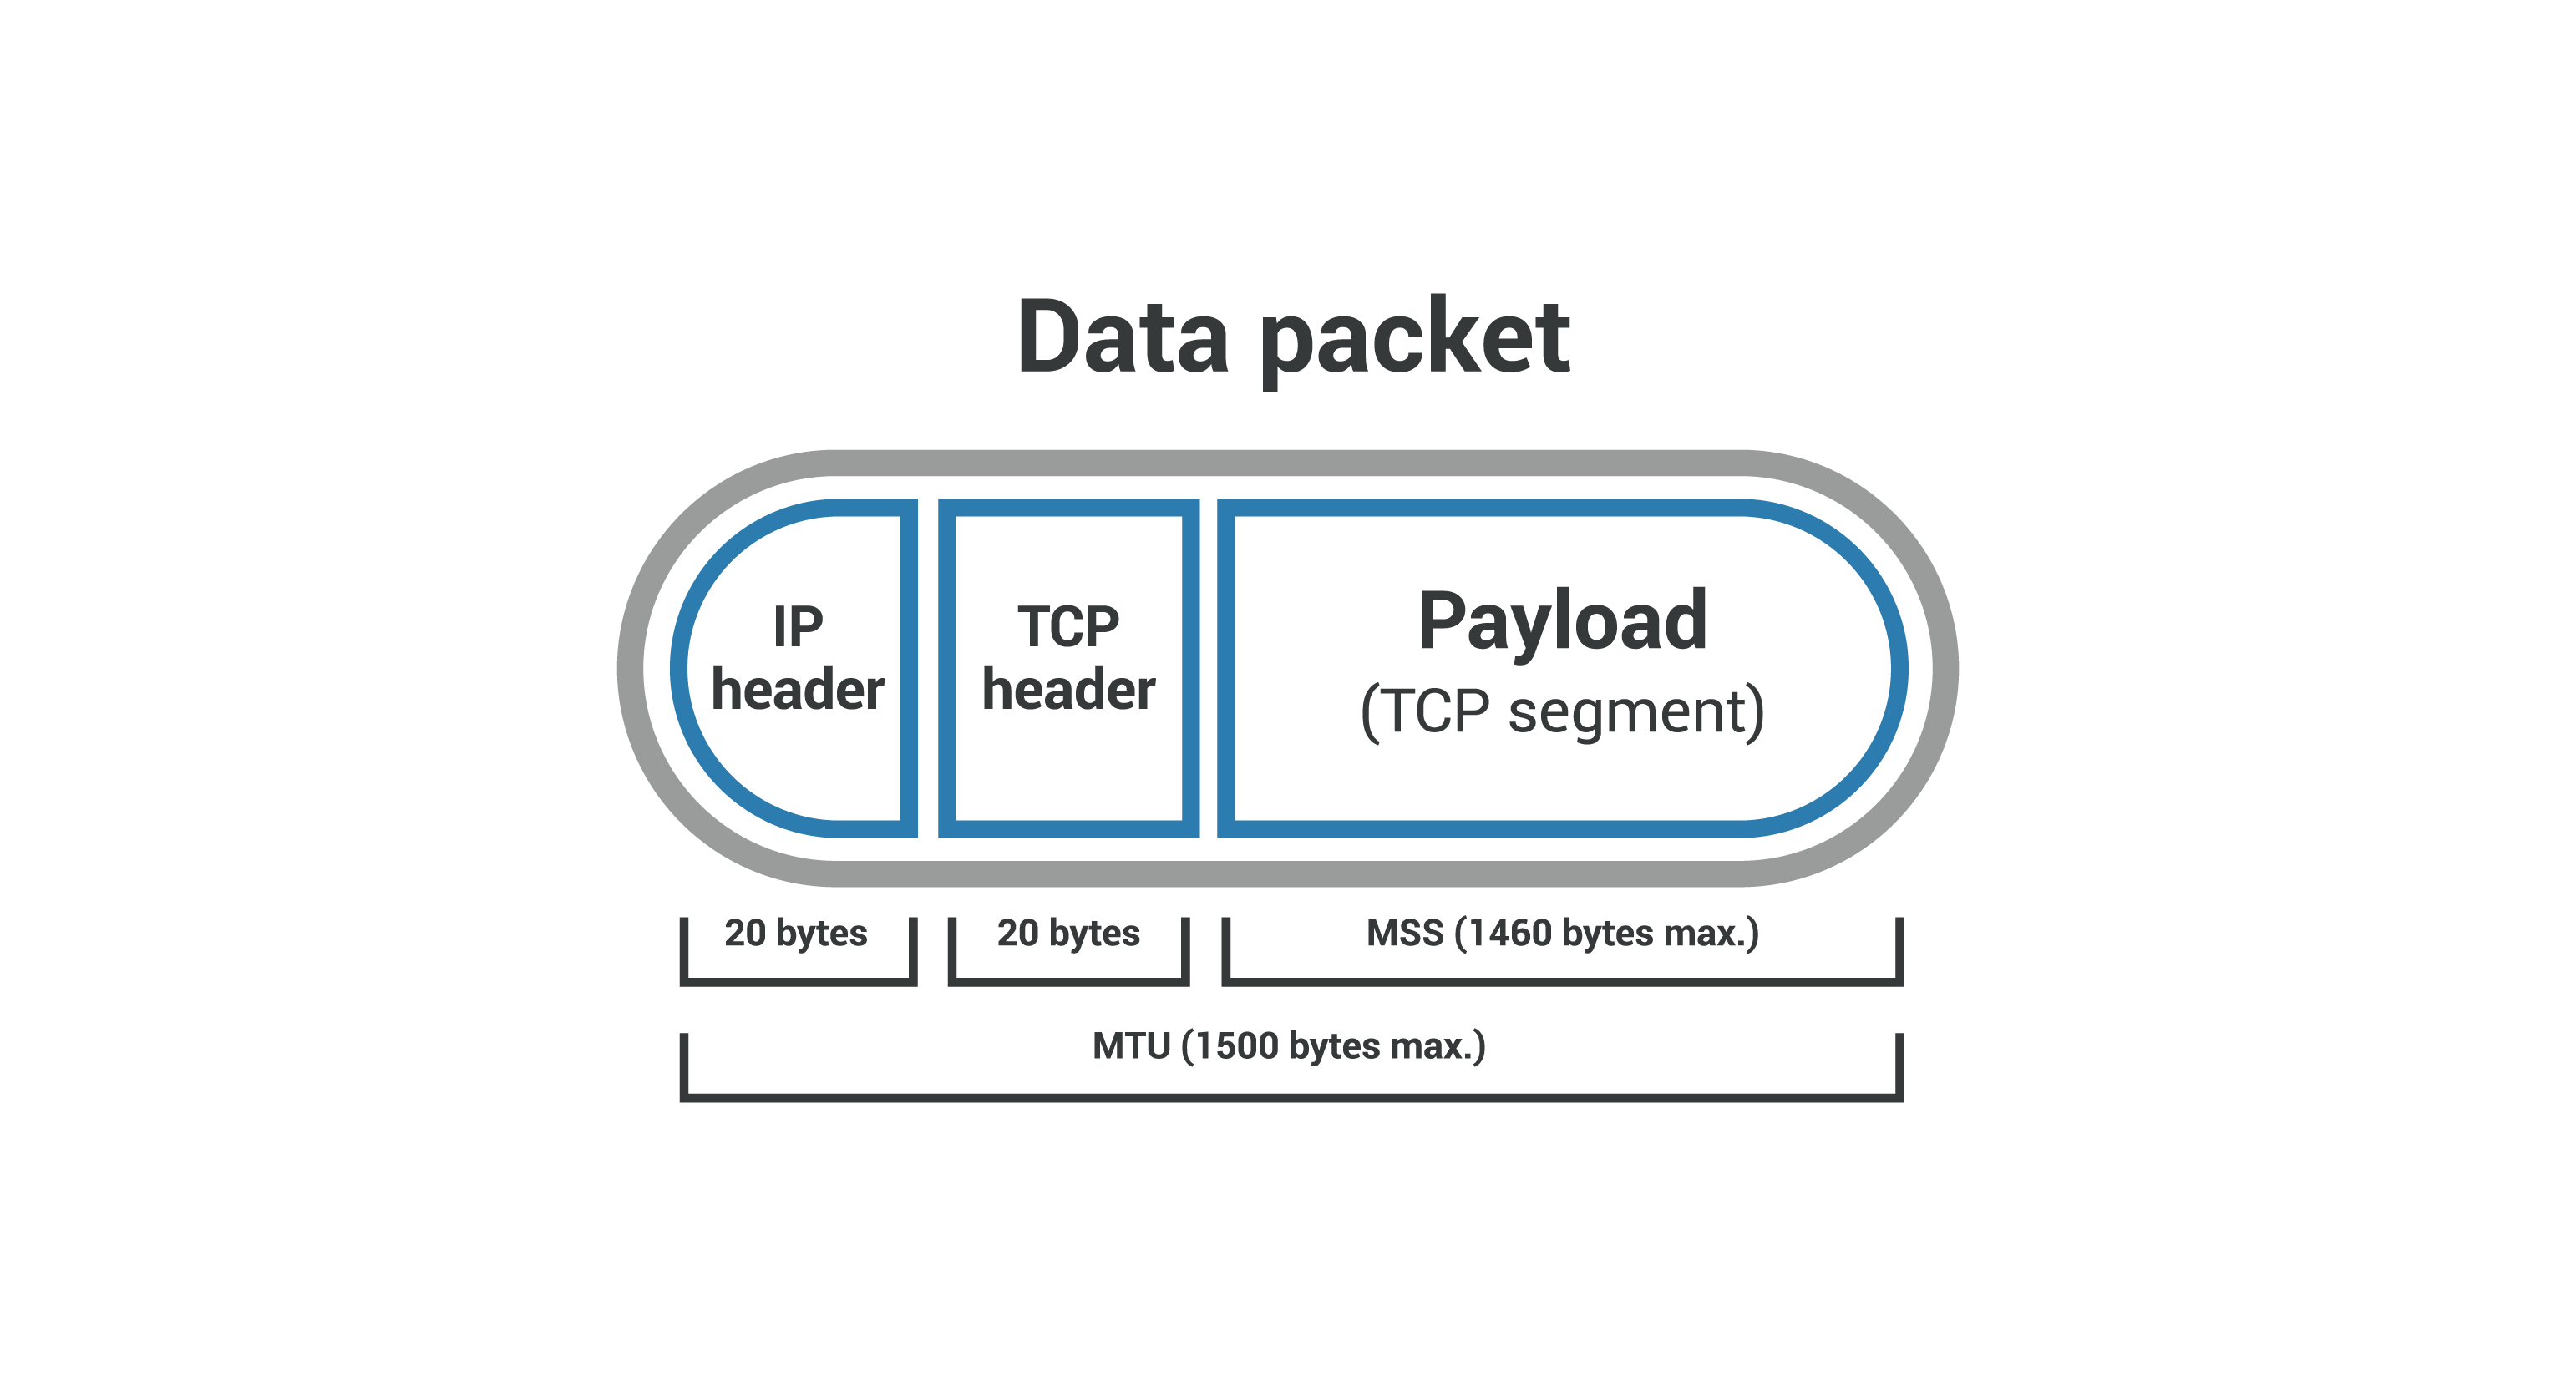
\includegraphics[width=1\textwidth]{Pictures/packet.png}
	\vspace{-60pt}
	\caption{Dátový balíček \cite{MSS}}
	\label{pic:Packet}
\end{figure}

Riešením bolo použitie vyrovnávacej pamäte o veľkosti 2\textsuperscript{10} bytov a postupné prijímanie dát zo sieťového prúdu pomocou cyklu. Gro tohto postupu je zobrazené vo výpise \ref{src:Stream}.
\vspace{10pt}
\begin{lstlisting}[label=src:Stream,caption={Postupné čítanie dát zo sieťového prúdu}]
TcpClient client = reciever_Listener.AcceptTcpClient();
NetworkStream nwStream = client.GetStream();

while ((i = nwStream.Read(buffer, 0, buffer.Length)) != 0)
{
    data += Encoding.ASCII.GetString(buffer, 0, i);
}
\end{lstlisting}
\vspace{5pt}

Mojou poslednou úlohou v časti reportovacieho systému na strane hry, ktorá prišla ako požiadavka od programátorov bolo pridať možnosť odosielať reporty priamo z editoru bez nutnosti mať spustenú hru. Typický prípad použitia bolo nahlasovanie chýb nájdených popri práci s náhľadom scény. Väčšina kódu bola prebratá z vyššie popísanej časti, museli byť však zmenené niektoré postupy. 

Odchytávanie klávesovej skratky bolo tentoraz realizované natívnym postupom zabudovaným do editora Unity. Stačilo vytvoriť statickú metódu \textit{CreateReport} a nad jej definíciu pridať atribút \enquote{MenuItem} ako znázorňuje výpis \ref{src:UnityReport}. To vyústi k vytvoreniu zástupcu tejto metódy v hornom paneli editora. Pozícia metódy v paneli je určená zadanou cestou v parametri atribútu \enquote{MenuItem}. Za túto cestou je potom možné pridať ľubovoľnú klávesovú skratku, ktorá túto akciu vyvolá.
\vspace{10pt}
\begin{lstlisting}[label=src:UnityReport,caption={Odchytenie stlačenia klávesovej skratky v editore Unity}]
[MenuItem("Tools/HBT/Reporting/Create report #F11")] // # -> Shift
static void CreateReport()
{
    // body...
}
\end{lstlisting}
\vspace{5pt}

Pôvodný postup vytvorenia snímky obrazovky pomocou metódy \textit{CaptureScreenshotAsTexture} bolo nutné nahradiť metódou \textit{ReadScreenPixel}, ktorá ale potrebuje vedieť presnú lokáciu a rozmery okna. Získať tieto údaje sa mi nakoniec podarilo až volaním C++ metód z user32.dll. Počas testovania na 4K monitore sa ukázalo, že tento prístup nevhodne vyhodnocuje veľkosť okna s nastaveným škálovaním v OS Windows. Toto bolo nutné upraviť ručne, čo ukazuje výpis \ref{src:DLL}.
\vspace{10pt}
\begin{lstlisting}[label=src:DLL,caption={Získanie veľkosti okna Unity editoru}]
[DllImport("user32.dll")]
private static extern bool GetWindowRect(IntPtr hwnd, ref Rect rectangle);
[DllImport("user32.dll")]
private static extern IntPtr GetActiveWindow();

private struct Rect {
    public int Left { get; set; }
    public int Top { get; set; }
    public int Right { get; set; }
    public int Bottom { get; set; }
}

private static Rect GetUnityBounds() {
    Rect unityWindowBounds = new Rect();
    float scale = Screen.dpi / 96;

    GetWindowRect(GetActiveWindow(), ref unityWindowBounds);

    unityWindowBounds.Right = (int)(unityWindowBounds.Right / scale);
    unityWindowBounds.Bottom = (int)(unityWindowBounds.Bottom / scale);
    
    return unityWindowBounds;
}
\end{lstlisting}

Na strane Windows Forms aplikácie implementovanej do nástroja HoboThor bolo nutné najskôr vytvoriť sadu tried a enumov, ktoré by po serializácií/deserializácií presne kopírovali štruktúru projektu či reportu s ktorou pracuje služba Mantis Bug Tracker. Následne bolo nutné navrhnúť užívateľské rozhranie. To prechádzalo iteratívnymi zmenami na základe spätnej väzby až do svojej finálnej podoby znázornenej na obrázku \ref{pic:Report}.

\begin{figure}[!htbp]
	\centering
	\setlength{\fboxsep}{0pt}
	\setlength{\fboxrule}{1pt}
	\fbox {
		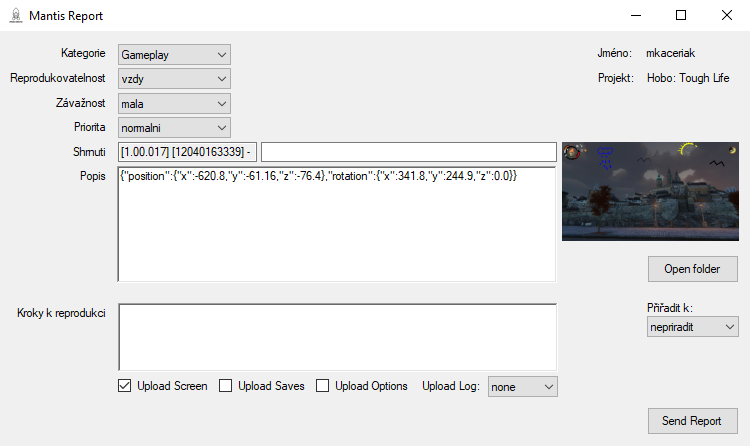
\includegraphics[width=.98\textwidth]{Pictures/report.png}
	}
	\caption{Užívateľské rozhranie aplikácie Mantis Report}
	\label{pic:Report}
\end{figure}

Po spustení aplikácie sa načíta uložená snímka obrazovky a zobrazí sa v náhľadovom okne na pravej strane. Vzhľadom na to, že v dobe spúšťania tento obrázok ešte nemusí byť plne k dispozícií je táto funkcionalita realizované v separátnom vlákne pomocou tzv. \enquote{Background Workera}. Ten v cykle prehľadáva zložku s reportom kvôli prítomnosti obrázku a až následne, keď je k dispozícií ho zobrazí.

Po načítaní dát z report zložky do polí \enquote{Shrnutí} a \enquote{Popis} sú odoslané dve GET žiadosti na server. Prvá požaduje dáta o užívateľovi, ktorému náleží príslušný api kľúč odoslaný spolu so žiadosťou a druhá požaduje informácie o projekte. Medzi tieto informácie patria aj kategórie evidované pre daný projekt. Tie sú vložené do kombinovaného poľa \enquote{Kategorie}. Tento postup bol zvolený z dôvodu možných budúcich zmien v štruktúre kategórií na serveri. Ostatné kombinované polia boli vyplnené vopred pripravenými enumami. U nich sa žiadna budúca zmena nepredpokladá.

Užívateľ zadá dostupné informácie k nájdenej chybe a report odošle na server. Táto akcia zahŕňa získanie dát zo všetkých dostupných polí a následné vytvorenie inštancie triedy \textit{Issue}, ktorá tieto dáta zapúzdruje. Všetky prílohy určené na odoslanie sú potom uložené do príslušných polí bytov, prevedené na reťazce s kódovaním base64 obdobným postupom ako vo výpise \ref{src:Zip} a predané spomínanej inštancií.

V tomto momente bola aplikácia prakticky hotová ale z QA oddelenia prišla požiadavka na možnosť úpravy obrázka pred odoslaním bez nutnosti použitia externých nástrojov. Vytvoril som teda druhé okno pre túto aplikáciu, ktoré sa otvorí po kliknutí na náhľadový obrázok a umožňuje do neho kresliť. Toto okno je znázornené na obrázku \ref{pic:Paint}. 

\begin{figure}[!htbp]
	\centering
	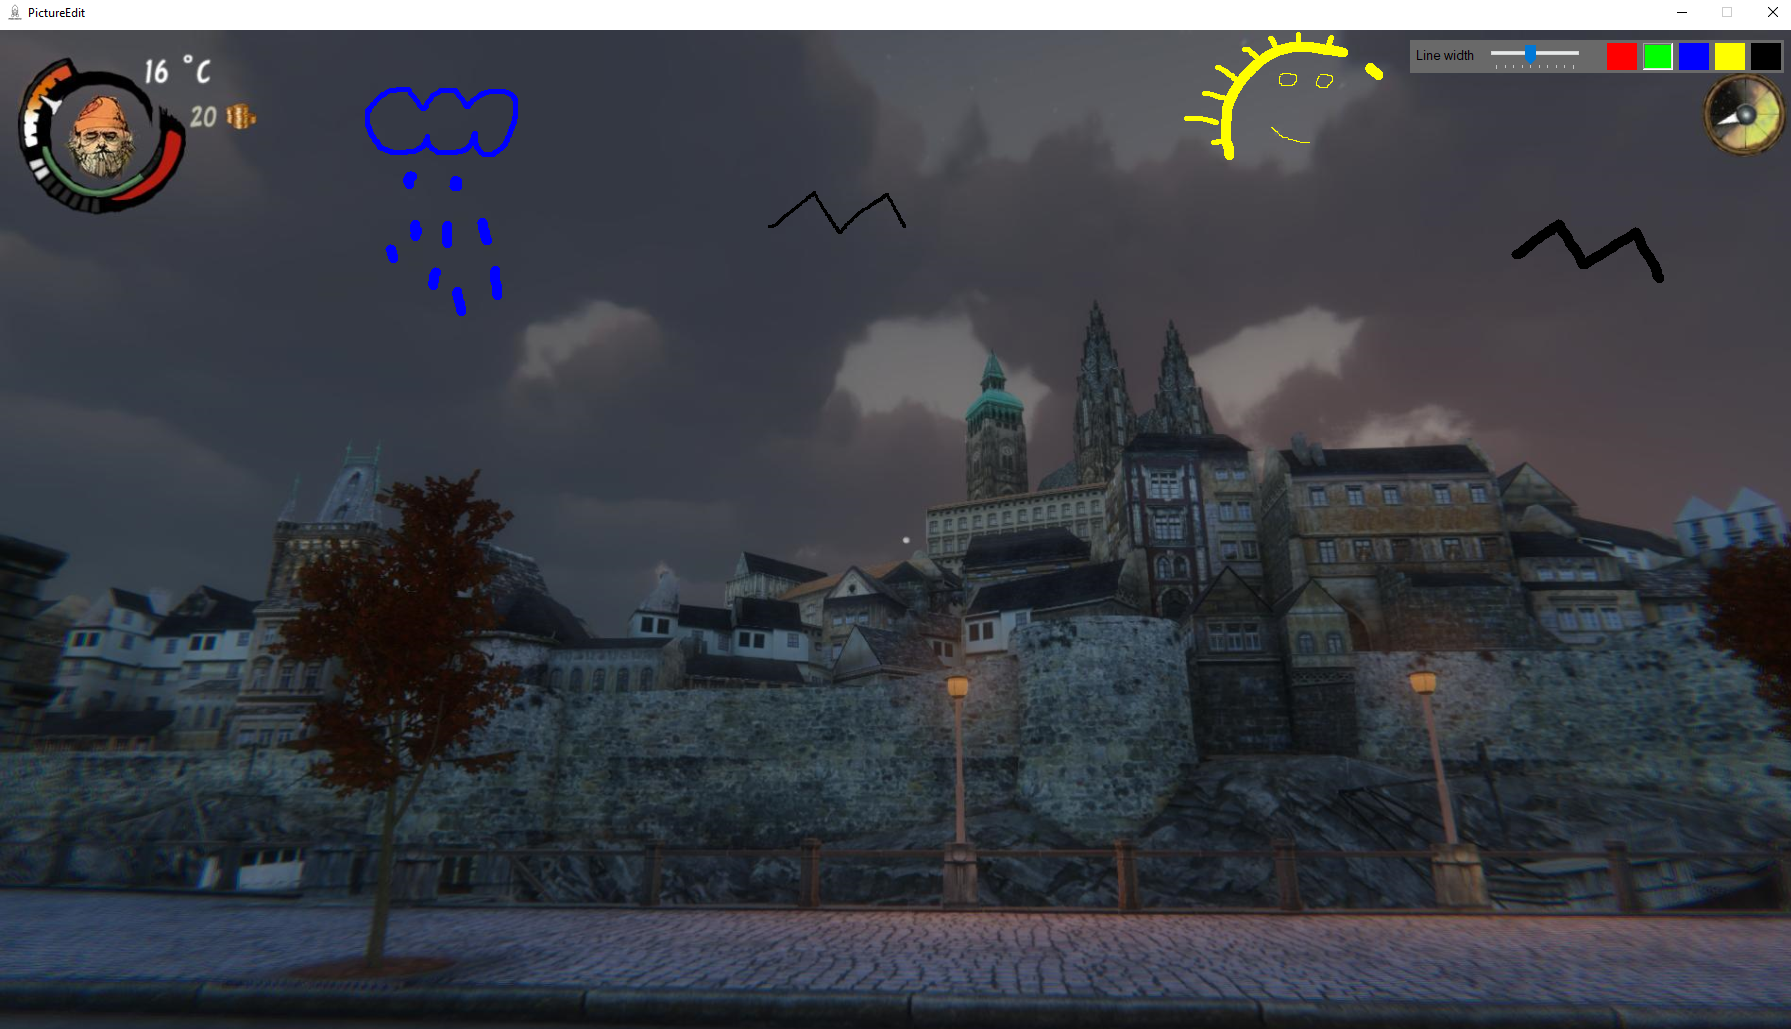
\includegraphics[width=1\textwidth]{Pictures/pictureEditBox.png}
	\caption{Okno úpravy obrázka aplikácie Mantis Report}
	\label{pic:Paint}
\end{figure}

Postupne bola pridaná podpora viacerých hrúbok a farieb čiar či tlačítko reset, ktoré slúži na návrat k pôvodnému obrázku. Zmeny v tomto okne sú spätne reflektované aj náhľadovým obrázkom v hlavnom okne reportovacej aplikácie. 

Na kreslenie bolo využité vlastné riešenie založené na udalostiach \textit{MouseDown}, \textit{MouseUp} a \textit{MouseMove}. Pri pohybe myši spolu so stlačeným ľavým tlačidlom dôjde k vykresľovaníu čiary medzi dvoma bodmi, čo sa od určitej frekvencie zaznamenávania bodov javí ako súvislý ťah. Tento postup je demonštrovaný vo výpise \ref{src:Paint}.
\vspace{10pt}
\begin{lstlisting}[label=src:Paint,caption={Implementácia kreslenia v prostredí Windows Forms}]
private void pictureBoxBcg_MouseDown(object sender, MouseEventArgs e) {
    moving = true;
    x = e.X;
    y = e.Y;
}

private void pictureBoxBcg_MouseMove(object sender, MouseEventArgs e) {
    if (moving && x != -1 && y != -1) {
        g.DrawLine(pen, new Point(x, y), e.Location);
        x = e.X;
        y = e.Y;
        pictureBoxBcg.Invalidate();
    }
}
private void pictureBoxBcg_MouseUp(object sender, MouseEventArgs e) {
    moving = false;
    x = -1;
    y = -1;
}
\end{lstlisting}
\subsection{Vytváranie \enquote{Patch notes} pre QA oddelenie (GitLogger)}
\label{sec:GitLogger}
\textbf{Časová náročnosť:} \\ Nasadenie: 3 dni.\\
\textbf{Úvod do problému:} \\ S blížiacim sa dátumom vydania hry sa zvyšuje aj frekvencia testovania a rýchlosť s akou pribúdajú opravy chýb. Medzi jednotlivými zostaveniami aplikácie býva nejaké časové obdobie - zvyčajne jeden týždeň. Toto obdobie je zakončené nahraním najnovšie zostavenej verzie hry na platformu Steam, kde ju môže QA oddelenie začať testovať. Informovanie testerov o najnovších zmenách a opravách môže byť pracné a náchylné na vynechanie niektorých dôležitých vecí. Mojou úlohou bolo tento proces pokiaľ možno čo najviac optimalizovať.\\
\textbf{Navrhované riešenia:} \\ Prvým navrhovaným riešením, ktoré sa už využívalo v niektorých vývojárskych nástrojoch bolo použitie knižnice, ktorá sa po zadaní správnych prihlasovacích údajov pripojí na Git server a prevedie prítomné \textit{commity} na štruktúru tried, s ktorou je potom možné ďalej pohodlne pracovať. Po preskúmaní tohto riešenia sa ukázalo, že jednotlivé knihovne nemajú vyriešenú podporu pripojenia na server pomocou protokolu SSH ale iba HTTPS, čo sa ukázalo ako veľký problém. Prišiel som teda s riešením, ktoré by si stiahlo \textit{commity} iba z lokálneho repozitára a to pomocou PowerShellu v OS Windows.  \\
\textbf{Realizácia:} \\ Po založení testovacieho projektu na platforme .NET bolo mojím prvým krokom zistiť, ako programovo spustiť rôzne skripty a príkazy v programe Windows PowerShell či klasickom príkazovom riadku. Postupne som narazil na triedu \textit{PowerShell} určenú presne pre tento prípad použitia. Pomocou tejto triedy som si vytvoril metódu, ktorá vie spustiť ľubovoľný príkaz a vrátiť jeho výsledok ako pole reťazcov. Táto metóda je znázornená vo výpise \ref{src:Shell}. 

Ako sa ukázalo, Windows PowerShell v predvolenom nastavení pre český jazyk nepoužíva kódovanie UTF-8, čo zapríčinilo nesprávnu interpretáciu znakov s diakritikou. Bolo nutné v nastaveniach systému v sekcií región túto voľbu ručne zapnúť, nakoľko je stále vo fáze vývoja.
\vspace{10pt}
\begin{lstlisting}[label=src:Shell,caption={Metóda na spustenie skriptu v programe Powershell}]
private string[] InvokePowershellScript(string gitCmd) {
    string[] results;
    using (PowerShell powershell = PowerShell.Create()) {
        powershell.AddScript($"cd {projectDirectory}");
        powershell.AddScript(gitCmd);

        results = powershell.Invoke().Select(r => r.ToString()).ToArray();
    }

    return results;
}
\end{lstlisting}

Po vyskúšaní rôznych preddefinovaných variant príkazu \textit{git log} som sa rozhodol zostaviť si vlastný príkaz, nakoľko mi žiadna preddefinovaná varianta úplne nevyhovovala. Hlavným dôvodom bola snaha čo najviac zjednodušiť následnú syntaktickú analýzu. Tento príkaz som sa rozhodol vytvárať dynamicky, aby sa sám aktualizoval po zmene premennej \textit{mainSplitter}. Ukážka tohto postupu je zobrazená vo výpise \ref{src:Log}.
\vspace{10pt}
\begin{lstlisting}[label=src:Log,caption={Generovanie vlastného príkazu git log}]
private const char mainSplitter = '&';
private string gitLog = "git log ";

public GitLogger() {
    gitLog += string.Format("--pretty=format:\"%an%{0}%ad%{0}%s\"" +
        " --date=format:'%d.%m.%Y'", ((int)mainSplitter).ToHex());
}
\end{lstlisting}

Následne bolo nutné v cykle prejsť všetky výsledky od najnovšieho \textit{commitu} až po \textit{commit}, ktorý značil posledné zostavenie hry interne dostupné na platforme Steam. Z týchto výsledkov sa odstránili všetky zlúčenia jednotlivých vetiev a ďalšie  \textit{commity}, ktoré neobsahovali ani opravy chýb ani novo pridané vylepšenia. Opravy boli značené tzv. \enquote{bugMarkerom} (@b) a vylepšenia tzv. \enquote{featureMarkerom} (@f). Tých mohlo byť v jednom \textit{commite} hneď niekoľko, preto bol na každý \textit{commit}, ktorý nejakú z týchto značiek obsahoval, aplikovaný regulárny výraz a jednotlivé časti boli ďalej spracovávané samostatne. Tento regulárny výraz zobrazuje výpis \ref{src:Regex}. Každá časť navyše mohla byť rozdelená na viacero menších častí rovnakého druhu pomocou znaku `;`. Jednotlivé elementárne časti boli následne štruktúrovane uložené do súboru.
\vspace{10pt}
\begin{lstlisting}[label=src:Regex,caption={Regulárny výraz na rozdelenie tela \textit{commitu}}]
var matches = Regex.Matches(body, string.Format("({0}|{1})[^@]*", bugMarker, featureMarker));
\end{lstlisting}

Pôvodný prípad použitia mal zahŕňať automatické otvorenie tohto súboru v predvolenom textovom editore a jeho ručné skopírovanie do programu Microsof Teams, ktorý sa používa na komunikáciu vo firme. Rozhodol som sa ale preskúmať možnosti automatizovaného odosielania správ v tejto službe a pokúsil sa implementovať lepšie riešenie.

Služba Microsoft Teams podporuje automatizované posielanie správ okrem iného aj pomocou tzv. \enquote{Webhooks}. Tie sa dajú nakonfigurovať priamo v užívateľskom rozhraní služby a to buď pre konkrétny kanál alebo konverzáciu. \enquote{Webhook} vygeneruje jedinečnú URL adresu, na ktorú je možné posielať POST žiadosti, ktoré sú spomenuté aj v sekcií \ref{sec:QACode}. Telo takejto žiadosti sa potom v aplikácií Microsoft Teams zobrazí ako správa odoslaná \enquote{Webhookom}. Dáta sú prenášané ako štruktúrovaný JSON reťazec. Okrem jednoduchých správ je možné posielať aj formátovaný text pomocou značkovacieho jazyka MarkDown, prípadne tzv. karty. 

Pomocou nástroja Postman som vo formáte JSON vytvoril dva návrhy takejto karty a nechal kolegov rozhodnúť o tom, ktorý sa nakoniec použije. Podľa zvoleného návrhu som následne implementoval triedu \textit{Message} tak, aby svojou vnútornou štruktúrou odpovedala štruktúre danej karty. 

Základnú kostru karty, ktorá sa počas vykonávania programu nebude meniť, som uložil do súboru. Pri každej novej POST žiadosti je tento súbor prečítaný a jeho obsah deserializovaný na novú inštanciu triedy \textit{Message}. Do tela správy sú vložené dáta získané z \textit{commitov} po syntaktickej analýze a následne je celá správa odoslaná do \enquote{WebHooku} metódu uvedenou vo výpise \ref{src:Shell}. Tento postup demonštruje výpis \ref{src:Message}. 
\vspace{10pt}
\begin{lstlisting}[label=src:Message,caption={Vytvorenie a odoslanie správy do služby Microsoft Teams}]
Message message = Message.FromJson(File.ReadAllText(pathToJSON));
Content content = message.Attachments[0].Content;

content.Title = header;
content.Sections[0].ActivityText = PrintListToJsonString(features);
content.Sections[1].ActivityText = PrintListToJsonString(bugs);

// cmdBegin == "Invoke-RestMethod -Method post -ContentType 'Application/Json; charset=UTF-8' -Body '";
string command = cmdBegin + Serialize.ToJson(message) + "' -Uri " + webHook;
string result = InvokePowershellScript(command)[0];
\end{lstlisting}

Metóda \textit{PrintListToJsonString} použitá vo výpise  \ref{src:Message} pridá do dát značky jazyka MarkDown, čím sa ešte upraví finálny vzhľad. Zároveň pomocou regulárneho výrazu \mbox{``\#\\d+``} nahradí všetky výskyty číselných reťazcov začínajúcich znakom `\#` za klikateľný odkaz na stránku konkrétneho reportu v službe Mantis Bug Tracker. To je užitočné v prípadoch keď \textit{commit} priamo opravuje nejakú nahlásenú chybu. Vytvorená karta je znázornená na obrázku \ref{pic:Logger}.

\begin{figure}[!htbp]
	\centering
	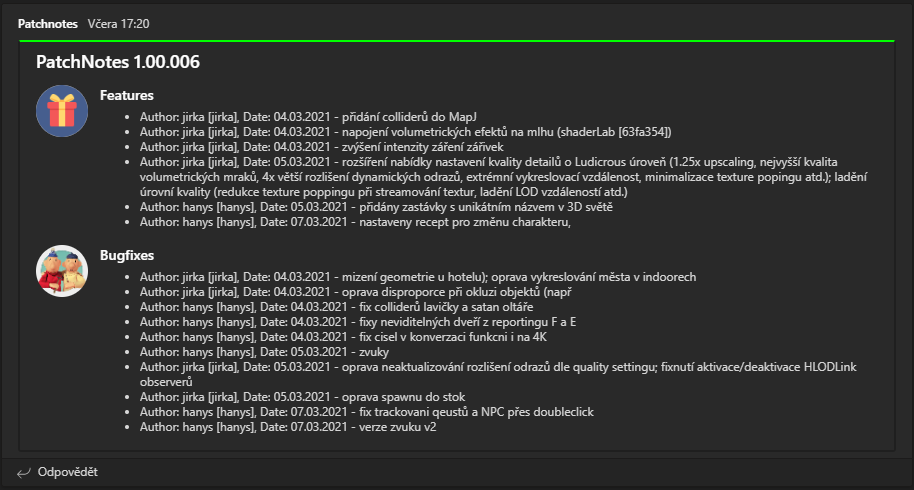
\includegraphics[width=1\textwidth]{Pictures/gitlogger.png}
	\caption{Vytvorená karta v aplikácií Microsoft Teams}
	\label{pic:Logger}
\end{figure}

Poslednou pridanou funkcionalitou bolo, aby sa táto karta neposielala pri každom zostavení hry na serveri ale iba vtedy, keď je to skutočne žiadúce. Aplikácia teda prečíta obsah súboru BuildSettings.asset a ak v ňom nájde reťazec ``sendPatchNotesToTeams: 1`` vykoná odoslanie. V opačnom prípade sú dáta len štruktúrovane zapísané na disk. Súbor BuildSettings.asset je podrobne popísaný v sekcií \ref{sec:BuildServer}.

Aplikácia bola nasadená ako externý súbor, ktorý je spustený službou Gitlab CI/CD bližšie popísanou v sekcií \ref{sec:GitLab}.
\subsection{Automatizované zostavenie hry na serveri (Build Server)}
\label{sec:BuildServer}
\textbf{Časová náročnosť:} \\ Nasadenie: 6 dní.\\
\textbf{Úvod do problému:} \\ Ako som spomenul v sekcií \\
\textbf{Navrhované riešenia:} \\ Nakoľko bola \\
\textbf{Realizácia:} \\ Pri preskúmavaní mož
\section{Optimalizácia a prevod hry na ďalšie platformy}
\label{sec:Port}
\section{Ostatné projekty}
\label{sec:Others}
asd
% End of section 4

% Section 5
%\chapter{Postup riešenia zadaných projektov}
%\label{sec:Processes}
%adasd
% End of section 5

%d) Teoretické a praktické znalosti a dovednosti získané v průběhu studia uplatněné studentem v průběhu odborné praxe.
%e) Znalosti či dovednosti scházející studentovi v průběhu odborné praxe.
%f) Dosažené výsledky v průběhu odborné praxe a její celkové zhodnocení.

\printbibliography[title={Literatúra}, heading=bibintoc]
\end{document}
